\documentclass{mai_book}

\defaultfontfeatures{Mapping=tex-text}
\setdefaultlanguage{russian}
	
\begin{document}

\newpage
%\lhead{\small\textit{$I-4.8$ \quad Настраиваемый модуль генератора биекций}}
%\rhead{91}
\begin{center}
\small\textbf{Реализация генератора биекций (Продолжение)}
\end{center}
\dotfill

\begin{lstlisting}[mathescape=true]
    typedef Source Source_Interval; //range in SOURCE_MIN .. SOURCE_MAX
    typedef Target Target_Interval; //range in Traget_Min .. TARGET_MAX
    Bijection Sigma = Create_Bijection(SOURCE_MIN, SOURCE_MAX); //range in Source_Interval
    Source_Interval Source_Index = SOURCE_MIN;
    Target_Interval Target_Index = TARGET_MIN;
    if (Sigma.Length != TARGET_MAX - TARGET_MIN + 1) {
        fprintf(stderr, "Not_A_Bijection");
        return BIJECTION_ERROR;
    }
    for (;;) {
        Set_Index(Sigma, Target_Index);
        if (Source_Index == SOURCE_MAX) {
            break;
        }
        Source_Index++; Target_Index++;
    }
    return Sigma;
}
void Successor_Of(Bijection The_Bijection, 
                  Signature With_Signature) {
    Positive Length = 1;
    Source First_Index;
    Source Ascending_Index, Descending_Index;
    for(Source i = The_Bijection.First; i <= The_Bijection.Last; i++) {
//Get has signature 'Source * Get(Bijection The_Bijection, Source Index)'
        if (*Get(The_Bijection, i) > *Get(The_Bijection, i + 1)) {
            Length++;
        } else {
            First_Index = i;
            break;
        }
    }
    
    if (Length == The_Bijection.Length) {
        fprintf(stderr, "Bijection_Overflow");
        return;
    }
    
    Ascendong_Index = First_Index + 1; Descending_Index = The_Bijection.Last;
    while (Ascending_Index < Descending_Index) {
        Swap(Get(The_Bijection, Ascending_Index), 
             Get(The_Bijection, Descending_Index));
        Ascending_Index++; Descending_Index--;
    }   
\end{lstlisting}

Первая функция, включенная в тело цикла,есть функция
\textit{Minimal\_ Bijection}. Её реализация требует особой заботы, если хотим\linebreak избежать переполнения индексов и иметь возможность осуществлять\linebreak те или иные проверки.

Начинают с определения двух подтипов, которые точно соответ- \linebreak ствуют целым интервалам исходного и конечного множеств биекции.\linebreak Эти два типа позволяют очень точно контролировать множество воз- \linebreak можных значений локальных переменных, а также проверять прежде \linebreak всего, что интервалы действительно могут быть подвергнуты биекции.\linebreak С этой проверки и начинается функция, и, возможно возбуждается\linebreak исключение \textit{Not\_ A\_ Bijection}. Если все указано с этой точки зрения,нуж-

\begin{wrapfigure}{i}{0.5\textwidth}
for (i==\textit{Sigma'Range})\{

   while(1)\{
   
   \textit{Sigma(i)}==i;\}\}
\end{wrapfigure}

  \noindent но предпринять ещё другие меры предосторожности; простой цикл, записанный слева не может быть использован в случаях несоответствия типов 

Нужно напротив пройти "вручную" по элементам исходного и ко-\linebreak нечного множеств, внимательно проверяя число осуществленных итера-\linebreak ций. Для этого используйте две переменные \textit{Source\_ Index} и \textit{Target\_ Index},\linebreak придавая им изначально наименьшее соответственно ис-\linebreak ходного множества и множества конечного и просматривая каждое из \linebreak этих двух множеств. Цикл заканчивается, когда одна из этих пере-\linebreak менных достигнет своего максимального значения (другая переменная \linebreak достигает своего максимального значения одновременно).\newline 

Принимая во внимание сказанное в предыдущем разделе,заключа-\linebreak ем, что реализация функции \textit{Successor} не требует дополнительных объ-\linebreak яснений. Однако отметим присутствие \textbf{Pragma}: в этой процедуре часто \linebreak бывает необходимо делать обмен значениями двух элементов таблицы,\linebreak поэтому естественно определить процедуру \textit{Swap}, которая это делает.\linebreak Пригма \textit{Inline}, которая применена к этой процедуре, означает, как это \newline 
\newpage
%\lhead{\small\textit{$I-4.8$ \quad Настраиваемый модуль генератора биекций}}
%\rhead{93}

показано в разделе 4.3, что нужно заменить обращение к процедуре\linebreak \textit{Swap} развертыванием "в линию" её тела. Совершенно очевидно, что\linebreak это указание не может применяться к рекурсивной подпрограмме. 

\section{Заключение}

\begin{flushright} 
\textbf{\dots as long as there were no machines, programming was no problem \\ at all; when we had a few weak computers, programming became \\ a mild problem, and now we have gigantic computers, programming\\ has become an equally gigantic problem. In this sense the electronic\\ industry has not solved a single problem, it has only created them - \\ it has created the problem of using its products. To put it in another\\ way:  as the power of available machines grew by a factor of more\\ than a thousand society's ambition to apply these machines grew in\\ proportion, and it was the poor programmer who found his job in this\\ exploded field of tension between ends and means\dots}\footnote{\dots пока не было машин, программирование вовсе не было проблемой; когда у нас появилось некоторое число слабых компьютеров, программирование стало представлять некоторую проблему, а теперь, когда мы имеем гигантские компьютеры, программирование стало столь же гигантской проблемой. В этом смысле электронная индустрия не решила ни одной проблемы, она только создала их - она создала проблему использования своей продукции. Другими словами: как только мощь доступных машин возросла более, чем в тысячу раз, так общество захотело использовать их в той же пропорции, и бедному программисту пришлось трудиться в этой стремительно расширяющейся области напряжения между целями и средствами \dots

                                                                     Э.В.Дейкстра, Смиренный программист (1972)}
\\
\ \newline
\textbf{Edsger W. Dijkstra, The humble programmer (1972 [66])}
\end{flushright}

Сделаем маленькое отступление. Около четверти века назад Дейкс-\linebreak тра [65] опубликовал статью "\textit{Go to statement considered harmful}" , в \linebreak которой он вскрывал недостатки команды безусловного ветвления. Не-\linebreak сколько лет спустя Вирт ввел язык Паскаль, который установил затем\linebreak свою диктатуру в обучении более, чем на десять лет. Этот длитель- \linebreak ный период ригоризма структур управления позволил структурному \linebreak программированию завоевать свои титулы и лавры и был совершен-\linebreak но необходим , чтобы умерить беспорядочное разбухание информатики.\linebreak Однако некоторые авторы, и среди них Кнут (\textit{Structured programming \linebreak  with goto statements}), настаивали на запрещении более гибкого сти-\linebreak ля программирования, такого, за который ратовали Дейкстра, Хоар \linebreak и Дал [58]\: или\:\: Вирт [182]\:. Но,\: как\: говорит\:\: Кнут [98]\: :  " \dots$~$\textit{During\: the}

\pagebreak
%\lhead{94}
%\rhead{\small\textit{$I-5$ \quad Заключение}}

\noindent\textit{programming, because I could' not bear to be found guilty of writing unstruc-\linebreak
tured programs }" \footnote[2]{"\dots в 70-е годы я, как и все остальные, был вынужден принять идеи структурного программирования, так как я не мог допустить, чтобы меня обвинили в написании неструктурных программ} , и однако, в течение многих лет никто не осмеливался заявлять миру в лицо, что он не программирует структурным образом ( в смысле Паскаля). 

Язык Ада, имеющий прямое родство с Паскалем (и, конечно, с другими языками), сделал заметно более гибкой позицию структурного программирования; зато в сравнении с Паскалем Язык Ада ещё крепче закрутил гайки относительно типов данных. С этой точки зрения он действительно суров! Но соображения, которые являлись определяющими при создании языка Ада, уходят гораздо дальше \textit{простых} задач программирования. Речь шла о построении стандартного языка, который, помимо всего прочего, позволил бы пользователям всех уровней обмениваться программами; мы же пока далеки от достижения этой цели. Мы полагаем, однако, что язык Ада обладает выразительной силой и четкостью, достаточными для того, чтобы служить основой для трансляции алгоритмов; но этого недостаточно \dots
\begin{flushright}


\parbox{11.5cm}{ 
\textit{\hspace*{15pt}Гордое восклицание "Пошло с первого раза!" обнаруживает в программировании черты искусства. Это утверждение, вполне понятное, но редко произносимое, означает следующее: написать программу, которая правильно работает с первого раза, возможно, но это не типично. Так как программисты, несомненно, стараются писать программы, которые идут с первого раза, встает вопрос: "если это возможно, почему это необычно?". Ответ  на этот вопрос двойной: во-первых, программировать трудно, и во-вторых, имеется имеется очень мало общих методов для разработки и написания хороших программ. Поскольку общих методов мало, каждый программист должен развивать свои собственные, часто с минимальным успехом. Успех этих методов зависит от способа, каким они адаптированы к конкретной задаче. По этой причине качество программ меняется не только от одного программиста к другому, но еще и от одной программы к другой у одного и того же программиста.}\newline
\ \newline
               \textit{Анри Ледгар, Пословицы программирования (1975[115])}
}
\end{flushright}
Программирование все еще является, в основном, техникой, требующей\linebreak умений, которые не приобретаются из книг; в нем отсутствует\linebreak строгость, которая приносит успех в математике. Как мы уже гово-\linebreak
рили, проверка программы имеющимися методами так же трудна, как и

\newpage
%\lhead{\small\textit{$I-5$ \quad Заключение}}
%\rhead{95}

\noindent математическое доказательство, если не позволять себе никакого отклонения от обозначений в смысле логики; это выше человеческих сил, даже если предположить, что все необходимые для этого средства существуют. Однако представляется вполне возможным убедить убедить разумного человека в том, что программа корректна, при условии ее представления в форме небольших модулей, поведение которых является понятным. Сопровождая эти модули просто проверяемыми утверждениями, мы делаем важный шаг в процессе передачи умений и навыков. Сколько мы изучили алгоритмов, постижение которых потребовало от нас длительных часов потому, что их авторы (которые, быть может, провели еще больше времени, составляя их) опубликовали их без всякого обоснования! Тогда как одно маленькое высказывание в нужном месте позволило бы быстро понять суть алгоритма. 

Что касается программирования, были так же сделаны попытки для упрощения передачи понимания программ от разработчика пользователю. Кнут[101], который является для нас объектом постоянных ссылок, работал в этом направлении, создавая свою систему документированного программирования \textbf{WEB}. Это направление, даже если оно не решает всех задач программирования --- в частности, оно не дает удовлетворительного решения проблемы архитектуры программ --- очень помогло нам на этапах программирования, которые мы уже прошли. Конечно, применение методологии программирования требует заметного напряжения, а время получения результата больше, чем обычно, что идет в разрез с философией программистов, для которых верхом изящества является возможность составить и выполнить программу одним нажатием кнопки. Но уже выбор языка Ада четко отделяет нас от этих программистов.

В дальнейшем на странице этой книги читатель найдёт сравнительно мало Ада-программ по сравнению с насыщенной ими первой главой. Причина, в основном, в недостатке места, которое было бы необходимо для представления этих программ. Однако мы реализовали большинство алгоритмов, которые представляем здесь, скорее для того, чтобы \textit{подтвердить} наши утверждения (что не составляет доказательства как такового), нежели для нахождения конкретных примеров или контрпримеров; и все эти алгоритмы представлены в форме, допускающей прямую реализацию. Сверх того, мы строго привержены принципу документирования, и в дальнейшем не найдётся - кроме тривиальных случаев - алгоритма, не сопровожденного небольшим инвариантом, что и делает жизнь приятной.
\newpage
\begin{center}
\textbf{Упражнения}
\end{center}
\paragraph { 1. Вычисление целого квадратичного корня}\ \newline

Если упражнение показывает, что классический метод Ньютона для вычисления квадратичного корня из действительных чисел равно применим в случае вычисления для целых чисел. Пусть $a$ ~--- целое строго положительное число; определим последовательность натуральных чисел ($a_{n}$) следующим образом: 

\begin{equation*}
a_0^2 \geqslant {a}  \text{    и     }  a_{n+1} = \left[\frac{a_n+\left[a/a_n\right]}{2}\right], \forall{n} \in {N}.
\end{equation*}

Можно считать, что если $a$ и $b$ --- целые положительные  числа, то [a/b] есть частное от деления $a$ на $b$ с помощью алгоритма Евклида. 

\subparagraph { a.}  Прежде всего, нужно точно сформулировать проблему. Что означает "$x$ есть целый квадратный корень из $a$"?
Для $x \in{N}$ доказать, что $\left[\left(x+\left[a/x\right]\right)/2\right]=\left[\left(x^{2}+a\right)/2x\right]$ . Для какой формы вычисления наиболее эффективны? 

\subparagraph {b.} Написать программу, которая вычисляет последовательность $(a_{n})$, начиная с некоторого значения $a$ , вводимого с клавиатуры, что позволяет наблюдать формирование последовательности и высказать правдоподобные предположения об условиях её сходимости. Затем можно написать программу, позволяющую проверить предположение на примере целых чисел, гораздо больших, чем в предварительных рассмотрениях. Продолжение упражнения состоит в доказательстве этого высказывания.

\subparagraph { c.} После изучения числовой функции $F\left(x\right)=\left(x+a/x\right)/2$, доказать, что последовательность $\left(a_{n}\right)$ обладает начальным строго убывающим сегментом, т.е. существует  целое $p$ такое, что для всякого $i>p$ имеет место $a_{i}>a_{i+1}$ и $a_{p}\leq{a_{p+1}}$ ( указание: показать, что $a_i^2>a\Rightarrow{a_{i}>a_{i+1}}$.

\subparagraph {d.} Показать, что  $\left(a_p+1\right)^2>a$. Вывести отсюда алгоритм вычисления целого квадратного корня из $a$. 

\subparagraph {e.} Изучить так же последовательность, определенную с помощью соотношений $a_0^2>a$  и 
$ a_{n+1} = \left[\frac{1+a_{n}+\left[a/a_{n}\right]}{2}\right]$.

\newpage

%\lhead{\small\textit{Упражнения}}

%\rhead{97}

\paragraph { 2. Целая часть функций}

\subparagraph { a.} Показать, что $\lfloor\sqrt{\lfloor {x }\rfloor}\rfloor=
\lfloor\sqrt{x}\rfloor$. В более общем случае показать, что если $f$ ~--- возрастающая непрерывная функция и если $f\left(x\right)\in{ N }\Rightarrow {x\in {N}}$ , то $\lfloor {f\left(\lfloor {x}\rfloor\right)}\rfloor=\lfloor{ f\left({x}\right)}\rfloor$

\subparagraph { b.} Если обозначить через $\lceil{x}\rceil$ наименьшее целое, превосходящее или равное $x$ (его{\it наибольшая}целая часть), то при каком условии $\lceil{\sqrt{\lfloor {x}\rfloor}}\rceil=\lceil{\sqrt{x}}\rceil$.

\subparagraph { c.} Пусть f ~-- -строго возрастающая непрерывная функция, такая что $f\left(x\right)\in{ N }\Rightarrow {x\in {N}}$ . Показать, что для всякого целого $x$ выполняется равенство $\lceil{f\left({x+1}\right)}\rceil=\lfloor{f\left({x}\right)}\rfloor$. 

\paragraph { 3. Вычисление целого корня n-й степени}\ \newline

Требуется для $a\in{N}$ вычислить $\lfloor{\sqrt[n]{a}}\rfloor$, где n ~--- целоe $ \geqslant{2}$. Метод Ньютона, примененный к уравнению $f\left({x}\right)=x^{n}-a=0$ на множестве действительных чисел, предполагает рассмотрение действительной функции $F\left({x}\right)=x-\frac{f\left({x}\right)}{f^\prime\left({x}\right)}= \frac{\left({n-1}\right)x^{n}+a}{nx^{n-1}}$. Тогда естественно для целых чисел рассмотреть последовательность $\left({x_{i}}\right)$,определённую как:

\begin{equation*}
\left({x_{i+1}}\right)=\lfloor\frac{\left({n-1}\right)x_i^n+a}{nx_i^{n-1}}\rfloor ~\text{для}~ i\geqslant{0}\quad\text{и}~ x_{0}\in{N}, ~x_o^n\geqslant{a}.
\end{equation*}

Руководствуясь упражнением 1 по вычислению квадратного корня в целых числах, доказать свойства последовательности $\left({x_{i}}\right)_{i\geqslant{0}}$ ( в случае необходимости ~-- с помощью программы) и вывести оттуда эффективный алгоритм, позволяющий вычислять $\lfloor\sqrt[n]{a}\rfloor$ (нужно особенно внимательно отнестись к выбору первого члена последовательности, если хотим, чтобы все вычисления оказались возможны). 

\paragraph { 4. Вычисление десятичных знаков числа $\sqrt{2}$}\ \newline

Это упражнение описывает элементарный метод, позволяющий генерировать один за другим десятичные знаки числа $\sqrt{2}$, который был использован Лалем в 1967 году для вычисления 19600 десятичных знаков у $\sqrt{2}$. С тех пор были сконструированы многочисленные другие методы. Читатель может обратиться к главе 5 из [135], где также присутствует вычисление других известных математических констант таких, как ${\pi}$ и ${e}$.

Пусть $ a_{0}$,$a_{1}$ $a_{2}$\dots $a_{k}$\dots ~--- разложение $\sqrt{2}$ по основанию $10~(\sqrt{2}=1,41421356 \dots)$. Положим 

\begin{equation*}
A_{k}=\left(a_{0}a_{1}\ldots a_{k}\right)_{10}=\lfloor{10^{k}\sqrt{2}}\rfloor \quad\text{и}\quad R_{k}=2\cdot10^{2k}-A_k^2=\left({10^{k}\sqrt{2}}\right)^{2}-A_k^2.
\end{equation*}

\newpage
	
	%\lhead{98}
	%\rhead{\small\textit{$I$ \quad Алгоритмика и программирование на языке Ада}}

\noindent Это означает, что $A_{k}$ есть целое число, образованное $k+1$ первыми цифрами $\sqrt{2}$, тогда как $R_{k}$ ~--- ошибка, обнаруживаемая при возведении этих двух величин в квадрат.

Показать, что $a=a_{k+1}$ есть наибольшее целое (заключительное между 0 и 1) такое, что $20aA_{k}+a^{2}\leq{100R_{k}}$, затем показать, что $R_{k+1}=100R_{k} - \left({20a_{k+1}A_{k}+ a_{k+1}^2}\right)$. Отсюда вывести алгоритм, позволяющий получить заданное число десятичных знаков $\sqrt{2}$. 

Хорошо видно, что$ A_{k}$ ~--- это неограниченное целое; такого ли$ R_{k}$?
Каким бы ни был ответ, дать порядок величины интервала, в котором \textit{находится} $R_{k}$.

\paragraph{5. Точный корень из целого числа}\ \newline

Для $n \in $N${^\star}$, обозначим $e\left({n}\right)$  наибольшее $k\geq{1}$ такое, чтобы $n$ было точной копией $k$-й степенью ($n$  всегда точная $k$-ая только для $k=1$); например, имеем $e\left({18}\right)=1$ и $e\left({248832}\right)=5$ , ибо $248832=12^{5}$. Это упражнение посвящено алгоритму вычисления пары $\left({r,e\left({n}\right)}\right)$  такой, что $n=r^{e\left({n}\right)}$ . Этот алгоритм часто используется перед алгоритмами разложения и не может поэтому использовать в своей реализации , по крайней мере,  каноническое разложение $n$.

\subparagraph { a.} Рассматривая каноническое разложение $n$ , установить несколько свойств функции $e:$N$^\star\rightarrow $N$^\star$. Показать, в частности, что $e\left({n^{q}}\right)=qe\left({n}\right)$.

\subparagraph { b.} Используя в качестве примитивов функции $\lfloor{\sqrt[m]{\hspace*{10pt}}}\rfloor$ $\left({m\geq {2}}\right)$ и функцию \textit{Next\_ Prime}, дающую простое число, следующее за данным целым, написать алгоритм (сопровождаемый доказательством), реализующий вычисление пары $\left({r,e\left({n}\right)}\right)$  для данного целого $n$. Каков диапазон целых $n$, поддающихся обработке с помощью набора простых чисел $<10^{3}$? 

\paragraph { 6. Порождение простых чисел}\ \newline

В этом упражнении устанавливаются алгоритмы, позволяющие последовательно находить нечетные простые числа, начиная с 3, которые будем обозначать $p_{1},p_{2},p_{3} \ldots $ ( в отличие от общепринятых обозначений , когда $p_{1}=2$). 

\subparagraph { a.} Написать алгоритм, который вычисляет $p_{1},p_{2},\ldots ,p_{n} $ для фиксированного $n$. Метод: определив все простые числа до $p_{k}$, выбирают в качестве кандидата $p_{k+2}$ и пробуют делить его на уже вычисленные $p_{i}$. Обязательно ли проверять делимость на все уже вычисленные простые числа?

\newpage
	
%\lhead{\small\textit{Упражнения}}
%\rhead{99}

\subparagraph { b.} Прежде чем читать формулировку этого вопроса, внимательно рассмотреть доказательство корректности (обеспечиваемое решением) алгоритма из предыдущего вопроса. В одном из циклов этого алгоритма для всякого нечетного $q$ осуществляется проверка $p_i^2>q$, что сводится к многочисленным бесполезным вычислениям квадратов. Можно без использования таблицы квадратов сократить этот счет, сохраняя две переменные, которые обозначают, соответственно, номер $i$ наименьшего простого $p_{i}$, квадрат которого превосходит испытываемые числа, и квадрат этого простого. Это возможно благодаря постулату Бертрана, который утверждает, что $p_{i+1}<2p_{i}$. Построить новый алгоритм, реализующий эту оптимизацию. 

\paragraph { 7. Правильный пятиугольник для всех (без Ферма и Гаусса}\ \newline

Показать, что $ \cos{\frac{\pi}{5}}=\frac{\phi}{2}$, где $\phi$ есть число золотого сечения. Вывести отсюда построение правильного пятиугольника с помощью циркуля и линейки. 

\paragraph { 8. "Двоичное" деление нацело}\ \newline
Цель этого упражнения ~--- вычисление частного и остатка от деления алгоритмом Евклида целого $a$ на целое $b$, используя только сложение, вычитание, умножение и деление на 2. 

\textbf{ a.} Выразить частное и остаток от евклидова деления $a$ на $b$ как функцию частного и остатка от евклидова деления $a$ на $2b$

\textbf{ b.} Написать алгоритм (рекурсивный) евклидова деления двух целых чисел, основанный на предыдущем свойстве. Этот алгоритм принимает на входе пару целых чисел и дает на выходе пару целых чисел. 

\textbf{ c.} Очень вероятно, что предыдущий алгоритм, если он прямо реализует свойства пункта $a$, даёт большую ошибку. Для примера попробуйте деление 31001 на 15 и представьте, что произошло бы, если бы все целые числа, с которыми проводятся вычисления, были заключены между $-2^{15}$ и $-2^{15}-1$. 

\textbf{ d.} Если алгоритм пункта $b$ не вызвал особых сложностей при работе с предыдущим примером написать итеративный алгоритм евклидова "бинарного" деления. 

\textbf{ e.} В конце упражнения рассматривается случай, наиболее вероятный для возникновения проблемы. В наиболее вероятном случае, когда возникает проблема, конец упражнения посвящен корректировки этой проблемы.  Предполагая, что $b_{0}\leq{a}$, показать, что два следующих алгоритма эквивалентны. 

\newpage
	
%\lhead{100}
%\rhead{\small\textit{$I$ \quad Алгоритмика и программирование на языке Ада}}
\iffalse
\noindent 
\begin{minipage}[t]{50mm}\parindent=2em
 
 
\fbox{$b\leftarrow{b_{0}}$;$k\leftarrow{0}$;\linebreak
While(1) \{\linebreak
$b\leftarrow{2\times{b}}$;$ k\leftarrow{k+1}$;\linebreak
  If(b>a) \{\linebreak
       Break;\}\}}\linebreak
\end{minipage} 
\hfill 
\begin{minipage}[t]{50mm} 
\fbox{$b\leftarrow{b_{0}}$;$k\leftarrow{0}$;\linebreak
While(b<=a/2) \{\linebreak
      While(1)\{\linebreak
$b\leftarrow{2\times{b}}$;$ k\leftarrow{k+1}$;\}\}\linebreak
$b\leftarrow{2\times{b}}$;$ k\leftarrow{k+1}$;}\linebreak
\end{minipage}
\fi


\begin{tabular}{p{6cm} p{6cm}}
\centering
\begin{lstlisting} [language=C,
					basicstyle=\small,
					aboveskip=-1em,
					belowskip=-1em,
					mathescape=false]			
_b = b[0]; k = 0;
do 
{
	_b *= 2;
	k++;
}
while (_a >= _b);
\end{lstlisting}&
\begin{lstlisting} [language=C,
					basicstyle=\small,
					aboveskip=-1em,
					belowskip=-1em,
					mathescape=false]
_b = b[0]; k = 0;
while (_b <= _a / 2) {
	_b *= 2;
	k++;
}
_b *= 2;
k++;
\end{lstlisting}
\end{tabular}

Отсюда вывести итеративный алгоритм евклидова деления двух целых чисел двоичными операциями, не содержащий ошибку, указанную в вопросе $c$. 

\paragraph { 9. Построение прямых линий методами DDA}\ \newline

DDA ~---аббревиатура, обозначающая \textit{Digital Differential Analyser}\footnote[1]{Цифровой дифференциальный анализотор.}, ~--- имя, данное методам построения геометрических фигур на основе дискретного разрешения (экран или графическое печатающее устройство), использующим только простые арифметические операции и целые числа ( в частности, эти методы никогда не применяются к вычислениям над числами с плавающей точкой). В дальнейшем предполагается, что "светящиеся" точки имеют целочисленные координаты. 
В этом упражнении описаны два алгоритма, позволяющие строить отрезки прямых на экране; предполагается, что прямые проходят через начало координат, имеют положительный наклон и находятся в первом квадранте; уравнение прямой имеет тогда вид $y=xv/u$, где $v>0$ и $u>0$ (вертикальные и горизонтальные прямые не составляют проблемы). 

\subparagraph { a.} Во всех этих алгоритмах можно считать $u$ и $v$ взаимно простыми. Почему?

\subparagraph { b.} Предположим сначала, что $u>v>0$ (т.е. отрезок, который требуется построить, находится в первом октанте); как следствие, рисуемый отрезок будет сформирован из маленьких горизонтальных отрезков. Разрешаются диагональные и горизонтальные движения точки на экране ( чисто вертикальные движения бесполезны, так как угловой коэффициент прямой меньше 1). Написать алгоритм, осуществляющий построение по предыдущим правилам. Указание: если $\left({x,y}\right)$ ~--- точка дискретной прямой, $y$ должен быть наилучшим приближением величины $vx/u$. 

\subparagraph { c.} Предположим только, что $u>0$ и $v>0$; требуется построить прямую в первом квадранте. Разрешаются только вертикальные и горизонтальные движения точки на экране ( не диагональные!). Написать алгоритм, который строит сегмент прямой $\left[{0,\left({u,v}\right)}\right]$, соблюдая 

\newpage
%\lhead{\small\textit{Упражнения}}
%\rhead{101}

правило перемещения и ставя точки как можно ближе к действительной прямой. Указание: поддерживать положение точки, аппроксимирующей прямую, в полосе, расположенной между двумя прямыми, параллельными искомой прямой и проходящими через точки $\left({-1/2,1/2}\right)$ и $\left({1/2,-1/2}\right)$ (см.рис.1) 

\begin{center}
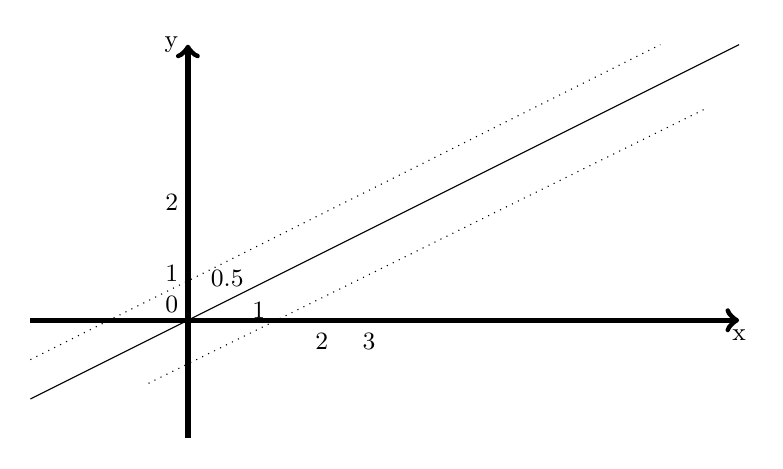
\begin{tikzpicture} [scale = 1]
\coordinate [label=left:\small{y}] (y) at (-3, 4);
\coordinate [label=below:\small{x}] (x) at (4, 0.5);
\coordinate [label=above:\small{0.5}] (0.5x) at (-2.5, 0.8);
\coordinate [label=above:\small{3}] (3x) at (-0.7, 0);
\coordinate [label=above:\small{2}] (2x) at (-1.3, 0);
\coordinate [label=above:\small{1}] (1x) at (-2.1, 0.4);
\coordinate [label=left:\small{0}] (0) at (-3, 0.7);
\coordinate [label=left:\small{1}] (1y) at (-3, 1.1);
\coordinate [label=left:\small{2}] (2y) at (-3, 2);
\draw[->, line width=2pt] (-5, 0.5) -- (4, 0.5);
\draw[->, line width=2p t] (-3, -1) -- (-3, 4);
\draw (-5, -0.5) -- (4, 4);
\draw[dotted] (-5, 0) -- (3, 4);
\draw[dotted] (-3.5, -0.3) -- (3.6, 3.2);
\end{tikzpicture}
\end{center}
\begin{center}
Рис.1. Аппроксимация прямой линии. 
\end{center}

\paragraph { 10. Построение окружности методами DDA}\ \newline

Речь идёт об ещё одном из методов DDA, который позволяет построить часть окружности в верхнем правок октане( каждой точке, построенной в этом октане, соответствует 1 точка в каждом из 7 других октанов). Ставится задача построить окружность с центром $O$ и радиусом $R$. Уравнение окружности известно: $x^{2}+y^{2}=R^{2}$, и в верхнем правом октане имеем: $y\in{\left[{R\sqrt{2}/2,R}\right]}$ и $ x\in{\left[{0,R\sqrt{2}/2}\right]}$. Два метода, представленные ниже, строят восьмую часть окружности как кривую $y=f\left({x}\right)$, а это означает, что на каждом шаге этих алгоритмов отыскиваются точки, расположенные на вертикали и минимизирующие (в смысле, который еще предстоит определить) удаленность по отношению к окружности. 

\subparagraph { a.} Показать, что если $\left({x,y}\right)$ есть точка на вертикали $x$, \textit{близкая} к действительной окружности, то одна из точек $\left({x+1,y}\right)$ или  $\left({x+1,y-1}\right)$ есть точка с целыми координатами, ближайшая к действительной окружности на вертикали $x+1$. В дальнейшем полагаем $f\left({x}\right)=\sqrt{R^{2}-x^{2}}$.
\newpage
	
	%\lhead{102}
	%\rhead{\small\textit{$I$ \quad Алгоритмика и программирование на языке Ада}}

\subparagraph { b.} Первый метод: для целой точки $\left({x,y}\right)$, аппроксимирующей точку $\left(x,f(x)\right)$, полагаем, что $y-1/2\leqslant{f\left({x}\right)}<y+1/2$. Установить алгоритм, который строит восьмую часть окружности. 

\subparagraph { c.} Второй подход: алгоритм Брезенхама (см. [38]) использует для построения дискретной окружности точки с целыми координатами, ближайшие к окружности в следующем смысле:  если $P=\left({x,y}\right)$ ~--- точка дискретной окружности, то из двух точек  $P_{1}=\left({x+1,y}\right)$ и  $P_{2}=\left({x+1,y-1}\right)$ выбирают ту, которая минимизирует расстояние до окружности. 

Это правило могло бы привести к исключительно сложным вычислениям, если бы Брезенхам не доказал (это нужно будет еще доказать)следующее свойство, которое мы принимаем : с предыдущими обозначениями и предложениями минимизировать разность между квадратами длин $OP_{i}$ и $R$, что позволит минимизировать разность между этими же длинами. После этого замечания составить алгоритм, который строит окружность Брезенхама во втором октане. Какие замечания можно сделать при сравнении полученного алгоритма с тем, который был составлен в вопросе $b$.

\paragraph { 11. Сложность возведения в степень}\ \newline

Цель этого упражнения ~--- показать, что всякий алгоритм вычисления $P=x^{n}$, использующий только умножение (как алгоритмы, представленные в книге), имеет минимальную сложность $\log_{2}{n}$. В этом исследовании нас интересует только число перемножений; процесс же счета может быть схематично представлен следующим образом:
%\begin{flushleft}
\begin{equation*}
\begin{split}
P_{1}&=y_{1}z_{1}, \text{ где } y_{1}z_{1} \in{\{1,x\}},\\ 
P_{2}&=y_{2}z_{2}, \text{ где } y_{2}z_{2} \in{\{1,x,P_{1}\}},\\
\vdots\\
P_{t}&=y_{t}z_{t}, \text{ где } y_{t}z_{t} \in{\{1,x,P{1},P{2}, \dots\,P{t-1}\}};\\
\end{split}
\end{equation*}
%\end{flushleft}
здесь $t$ есть сложность алгоритма. 

\paragraph { 12. Последовательность Фибоначчи и золотое сечение}\ \newline

Числа Фибоначчи определены с помощью соотношений: $F_{0}=0$, $F_{1}=1$ и $F_{n}=F_{n-1}+F_{n-2}$. Они тесно связаны с числом золотого сечения $\phi\approx{1,618}$, которое является положительным корнем уравнения $x^{2}-x-1=0$; второй корень этого уравнения традиционно обозначается  $\phi$. 

\newpage
%\lhead{\small\textit{Упражнения}}
%\rhead{103}

\subparagraph { a.}Установить соотношения, возможно проще выражающее $F_{n}$ как функцию от $\phi$ и $\hat{\phi}$. Указание: установить свойства порождающего ряда 
$F={\sum_{}^{}}_{n\geq{0}}F_{n}X^{n}$ (или, иначе, производящей функции).

\subparagraph { b.}Представить $\phi^{n}+\hat{\phi}^{n}$ как функцию от чисел Фибоначчи. 

\subparagraph { c.} Записать $\phi^{n}$ как функцию от чисел Фибоначчи наиболее простым возможным способом. 

\paragraph { 13. Соотношения в последовательности Фибоначчи }

\subparagraph { a.} Рассмотрим матрицу $A=\begin{pmatrix}1 & 1 \\ 1 & 0 \end{pmatrix}$. Вычислить $A^{n}$. Отсюда вывести соотношения
\begin{equation*}
F_{n+1}F_{n-1}-F_n^2=\left({-1}\right)^{n} и F_{n+m}=F_{n}F_{m+1}+F{n-1}F_{m}.
\end{equation*}
\subparagraph { b.} Вычислить $f_{n}={\sum_{}^{}}_{k=0}^{n}F_{k}F_{n-k}$. Указание: каков общий член произведения двух формальных рядов?

\paragraph { 14. Линейные рекуррентные последовательности $k$-го порядка }

\subparagraph { a.} Исследовать последовательность целых чисел $\left({x_{n}}\right)$, определяемую соотношением $x_{n+2}=x_{n+1}+x_{n}$, где первые члены $x_{0}$ и $x_{1}$ ~--- произвольные фиксированные числа. Какую связь она имеет с последовательностью Фибоначчи? 
\subparagraph { b.} Фиксируется $k$ чисел $a_{0},a_{1},\dots, a_{k-1}$ и рассматриваются все линейные рекуррентные последовательности $k$-го порядка, т.е. определяемые соотношениями вида $x_{n+k}=a_{0}x_{n+k-1}+\dots a{k-1}x{n}$. Какая связь существует между этими последовательностями и матрицей Фробениуса
$$A= \begin{pmatrix} 
a_{0} & a_{1}&\dots    & a_{k-2}& a_{k-1} \\ 
1         & 0        & \dots  & 0           & 0\\
 0        & 1        & {}      & 0           & 0 \\
\vdots & {}      & {}      & {}          & \vdots \\
0         & 0        & {}      & 1           & 0
\end{pmatrix}?$$
Указание: найти базис пространства этих последовательностей.

\paragraph { 15.Дихотомия по Горнеру }\ \newline

Классический алгоритм дихотомического возведения в степень\linebreak основан на\: том\: факте, что\: если\: $n=n_{k}2^{k}+ n_{k-1}2^{k-1}+ \dots + n_{1}2^{1}+ n_{0}2^{0}$,\: то
\newpage
	
	%\lhead{104}
	%\rhead{\small\textit{$I$ \quad Алгоритмика и программирование на языке Ада}}

\noindent $x^{n}=x^{n_{k}2^{k}} x^{n_{k-1}2^{k-1}} \dots x^{n_{1}2^{1}} x^{n_{0}2^{0}}$; алгоритм действует, вычисляя  $x^{2^{i}}$ и\linebreak перемножая те из них, которые соответствуют ненулевым цифрам $n_{i}$. 

Существует другой способ использования разложения $n$ по основа-\linebreak нию 2, который состоит в применении для вычисления $n$ метода Горне-\linebreak ра, как многочлена, и использовании этого разложения для вычисле-\linebreak ния $x^{n}$. Например, для $x^{11}$ традиционным дихотомическим\linebreak способом, берут $ n=1\times{8}+0\times{4}+1\times{2}+1\times{1}$ и вычисляют 

\begin{equation*}
x, x^{2},x^{3},x^{4},x^{8},x^{11} \text{ возведением в квадрат и перемножением},
\end{equation*}
тогда как при дихотомии «по Горнеру» записывают $n= (\left({\left({1}\right)\times{2}+0}\right)\times$\linebreak
$\times{2}+1)\times{2}+1$ и вычисляют 

\begin{equation*}
x, x^{2},x^{4},x^{5},x^{10},x^{11} \text{ возведением в квадрат и перемножением}.
\end{equation*}
Упражнение посвящено созданию этого алгоритма возведения в сте-\linebreak пень «по Горнеру».


\subparagraph { a.} Рассмотрим многочлен $P=\sum_{i=0}^k a_{i}X^{i}$ и обозначим $ P_{i}=$\linebreak
$={\sum_{}^{}}_{j=1}^k a_{j}X^{j-i}$ Каковы $P_{0}$ и $P_{k}$? Какого соотношение между $P_{i}$ и $P_{i-1}$,\linebreak определяющее традиционный метод Горнера, используемый для вычи-\linebreak сления многочлена в некоторой точке? Вывести отсюда алгоритм вы-\linebreak числения многочлена $P$ в некоторой точке и указать число умножений и сложений, осуществляемых алгоритмом. 

\subparagraph { b.} Рассматривая запись величины $n$ по основанию 2 как вычисление некоторого многочлена $P$ в точке 2, вывести отсюда алгоритм вычисления $x^{n}$, точно следуя процессу вычисления «по Горнеру» этого многочлена. Для этого следует предполагать, что известны цифры числа $n$ по основанию 2. Полученный алгоритм не должен быть, очевидно, рекурсивным. 

\subparagraph { c.} Как можно действовать в предыдущем алгоритме, не зная бинарного разложения $n$, но зная, что $2^{k}\leq{n}<2^{k+1}$ (тут есть тонкость!).

\subparagraph { d.} Оценить сложность этого алгоритма количеством умножений, предполагая затраты на одно умножение постоянными. 

\paragraph { 16. Вычисление чисел Фибоначчи }

\subparagraph { a.} Написать эффективный алгоритм вычисления чисел Фибоначчи. Напомним, что числа Фибоначчи определяются последовательностью $F_{0}=0$, $F_{1}=1$ и $F_{n+2}=F_{n+1}+F_{n}$.

\newpage
%\lhead{\small\textit{Упражнения}}
%\rhead{105}
\subparagraph { b.} Используя соотношение между последовательностью Фибоначчи\linebreak ${\left({F_n}\right)}_{n\geq{0}}$ и числом золотого сечения $\phi$ или матрицей $\begin{pmatrix}1 & 1 \\ 1 & 0 \end{pmatrix}$, рассмо-\linebreak тренные в упражнении 12, написать эффективный алгоритм вычисле-\linebreak ния $n$-го числа Фибоначчи.

\subparagraph { c.} Прочитав решения предыдущего пункта и используя упражне-\linebreak ние 15, придумать другой алгоритм вычисления $F_{n}$, основанный на тех\linebreak же соотношениях. Является он более эффективным, чем предыду-\linebreak щий? 

\paragraph { 17.$\epsilon$-лексикографический порядок и законопеременный лексикографический порядок}\ \newline

Для заданного отношения порядка $\leq$ условимся использовать следу-\linebreak ющие обозначения:
\begin{equation*}
a\leq^{1}b \equiv^{def} a\leq^{b}  \text{и}   a\leq^{-1}b \equiv^{def} b\leq^{a}
\end{equation*}

Пусть $E$ и $F$ - два упорядочных множества и $\epsilon$ - отображение\linebreak $E$ в множество      
\{-1,1\}. Рассматривается отношение порядка, опреде-\linebreak ленное на $E\times{F}$ посредством 

\begin{equation*}
\left({x,y}\right)\leq{\left({x^{\prime},y^{\prime}}\right)} \Leftrightarrow^{def} x<x^{\prime} \text{или} x=x^{\prime} и y\leq^{\epsilon\left({x}\right)}y^{\prime}.
\end{equation*}
\subparagraph { a.} Проверить, что это отношение - действительно порядок; оно\linebreak называется $\epsilon$-\textit{лексикографическим}порядком. Что можно сказать, если\linebreak отношение порядка, заданные на $E$ и $F$, суть отношения линейного порядка? Какой порядок получем на $E\times{F}$, если функция $\epsilon$ тождественно равна 1?
\subparagraph { b.} Для $x\in{E}, x\times{F}$ есть подмножество множества $E\times{F}$, которое\linebreak можно рассматривать как "вертикальную плоскость". Сравнить поря-\linebreak док в $F$ и порядок на $x\times{F}$ (индуцированный на\linebreak $x\times{F}$ порядком на $E\times{F}$
\hspace*{-10pt}\subparagraph {c.} Каждому \textit{линейно упорядоченному}множеству $E,E=$\linebreak$\{{x_{0}<x_{1}<x_{2}<\dots}\}$, по определению поставим в соответствие функ-\linebreak цию $\epsilon$, заданную как 
 $\epsilon\left({x_{i}}\right)=\left(-1\right)^{i}$ и называемую \textit{сигнатурой}$E$. Для\linebreak данных двух \textit{конечных, линейноупорядоченных} множеств \textit{законочереду-\linebreak ющимся лексикографическим порядком}называется $\epsilon$-лексикографиче-\linebreak ский порядок на $E\times{F}$, где $\epsilon$ есть сигнатура $Е$. Каков первый элемент\linebreak в $E\times{F}$? Последний? Написать функцию следования в $E\times{F}$ Выразить\linebreak сигнатуру $E\times{F}$ как функцию сигнатур $E$ и $F$
 
\end{document}


  
